\chapter{kód}
\section{Vysvetlenie kódu}

Pre správne fungovanie zariadenia sme potrebovali veľa funkcií na spracovanie signálu z mikrofónu do formy, s ktorou by sme mohli pracovať.

\section{Zero()}

Prvá funkcia potrebná na analýzu signálu je funkcia zero(). Jej úlohou je nájsť nulovú hladinu, číslo okolo ktorého oscilujú hodnoty signálu prijatého z mikrofónu. Princíp je nasledovný: do pomocnej premennej sum ukladá 5000 nameraných hodnôt takým spôsobom, že ich sčítava dohromady. Na konci tohto cyklu vydelí konečné číslo počtom nameraných hodnôt, čím získame priemer, ktorý sa zároveň rovná nulovej hladine. Táto funkcia sa vykoná v setupe(). 

\begin{lstlisting}

void zero() {
  float sum=0;
  int x;
  int i=0;
 while ( i < 5000) {
  x=analogRead(ReadPin);
  sum=sum+x;
  i++;
  }
  zerolevel=sum/5000.;
  }

\end{lstlisting}

\section{Maxvolume()}

Ďalšou dôležitou funkciou je funkcia maxvolume(). Jej úlohou je na konkrétnych intervaloch zisťovať maximálnu hodnotu signálu. Túto hodnotu si drží uloženú v premennej u po dĺžku hľadania novej hodnoty na ďalšom intervale rovnakej dĺžky. Táto funkcia je pre analýzu signálu veľmi dôležitá lebo pomocou nej môžeme signál upraviť do formy, v ktorej budeme vedieť overovať či hlasitosť už prekročila nami určenú hladinu hlasitosti. 

\begin{lstlisting}

void maxvolume(int mic) {
  currentMillis = millis();
  Umaxval=zerolevel;
  if (mic>Umaxval) {Umaxval=mic;}
  if (currentMillis - startMillis >= period1)
  {
     u=Umaxval;
    startMillis = currentMillis;
    Umaxval=zerolevel;
  }
}

\end{lstlisting}


\begin{figure}[!tbh]
\centering
\fbox{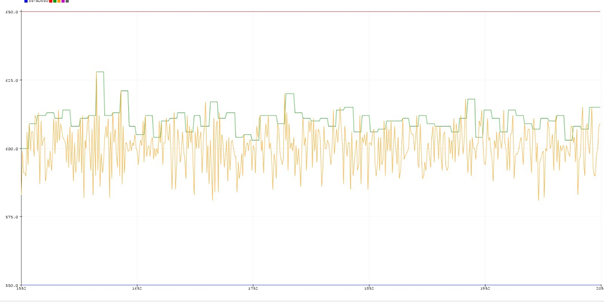
\includegraphics[width=\textwidth]{obr/graf1.png}}
\caption{Výstup mikrofónu pri intervale merania 20 ms.}\label{OBRAZOK 2.1}
\end{figure}

\begin{figure}[!tbh]
\centering
\fbox{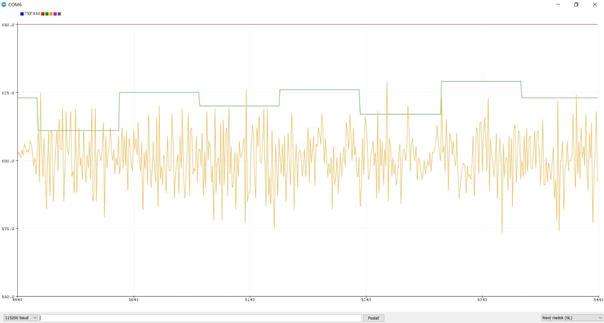
\includegraphics[width=\textwidth]{obr/graf2.png}}
\caption{Výstup mikrofónu pri intervale merania 100 ms.}\label{OBRAZOK 2.2}
\end{figure}


\section{Volume()}

Funkcia volume() slúži na zvyšovanie a znižovanie hlasitosti televízora. Kontroluje, či hodnota signálu (u) prekročila nami určenú maximálnu alebo minimálnu prípustnú hladinu. Ak táto situácia nastane počká určitý interval – period2 – a po jeho uplynutí znova overí podmienku. Toto slúži ako ochrana pred chybami, ktoré sa môžu vyskytnúť v priebehu signálu ale taktiež nám umožňuje nastavovať rýchlosť reakcie na zmenu hlasitosti. Ak podmienka platí aj po overení, zariadenie pomocou IR led pošle signál televízoru, ktorý hlasitosť buď zvýši alebo zníži.

 \begin{lstlisting}
void volume(int u){
 if (u < minval){
   currentmill = millis();
      if (currentmill - startmill >= period2)
         {
     digitalWrite(8, HIGH);
     IrSender.sendNEC(0x4,0x2,0);
     startmilll= millis();
   YieldDelay(100);
    digitalWrite(8, LOW);
  startmill = currentmill;
   }
  }
if (u > maxval ){
currentmill = millis();
if (currentmill - startmill >= period2)
     {
     digitalWrite(6, HIGH);
     IrSender.sendNEC(0x4,0x3,0);
    YieldDelay(100);
    digitalWrite(6, LOW);
     startmill = currentmill;
 }
}
}

\end{lstlisting}

Nasledujúce funkcie slúžia na ovládanie a nastavovanie parametrov programu pomocou potenciometrov.


\section{Volumelevel()}

Pomocou tejto funkcie si cez potenciometer dokážeme nastaviť aktuálnu výšku maximálnej (maxval) a minimálnej (minval) prípustnej hladiny hlasitosti bez toho by sme prepisovali program. V programe si musíme len nastaviť hodnoty, v ktorých sa budú môcť dané hodnoty pohybovať a maximálnu a minimálnu hodnotu získanú z potenciometra.

 \begin{lstlisting}
void volumelevel() {
  int MAXVAL_maxlevel = zerolevel + 60;
  int MAXVAL_minlevel = zerolevel + 10;
  int MINVAL_maxlevel = zerolevel + 30;
  int MINVAL_minlevel = zerolevel + 5;

  int minpot=0;
  int maxpot=660;
  float x=analogRead(LevelPin);

  maxval=((x/(maxpot-minpot))*(MAXVAL_maxlevel-MAXVAL_minlevel))+MAXVAL_minlevel;

  minval=((x/(maxpot-minpot))*(MINVAL_maxlevel-MINVAL_minlevel))+MINVAL_minlevel;
  }

\end{lstlisting}

\section{Reactiontime()}

Táto funkcia slúži na nastavovanie rýchlosti reakcie zariadenia na zmenu signálu z mikrofónu pomocou potenciometra v reálnom čase. Tak isto ako vo funkcii volumelevel() si v programe musíme nastaviť hodnoty, v ktorých intervale sa budeme pri nastavovaní pohybovať – maxperiod a minperiod. Tiež si nastavíme maximálnu a minimálnu hodnotu získanú z potenciometra.

  \begin{lstlisting}
void reactiontime () {
  int minpot=0;
  int maxpot=660;
  float x=analogRead(Period2Pin);

  int maxperiod = 5000;
  int minperiod = 500;

  period2 = ((x/(maxpot-minpot))*(maxperiod-minperiod))+minperiod;
  }

\end{lstlisting}

V loope programu teda len voláme dané funkcie až na zero() , ktorá je v setupe.